\documentclass[main.tex]{subfiles} % Subfile-Class


% ============================================================================== %
%                            Subfile document                                    %
% ============================================================================== %

\begin{document}

\section{Risikomanagement}

Das Risikomanagement wird nach der ALARP-Methode (\textit{engl. as low as
    reasonably possible}) durchgeführt. Dafür werden Risiken im ersten Schritt
identifiziert und anschliessend durch risikomindernde Massnahmen auf ein Niveau
reduziert, das ein angemessenes Mass an Sicherheit bietet. Die Bewertung
erfolgt im gesamten Team und basiert auf einer subjektiven Einschätzung zur
Erfüllung der Aufgabe. Ziel ist es, möglichst früh im Projektverlauf kritische
Punkte zu identifizieren und den Fokus auf diese zu legen. \

% -------------------------------------- Erläuterung Bewertung

\subsubsection*{Eintrittswahrscheinlichkeit (EW)}

Die Eintrittswahrscheinlichkeit ist ein Mass für die Wahrscheinlichkeit, mit
der ein Ereignis eintreten könnte.

\begin{table}[H] \begin{tabularx}{\textwidth}{|>{\centering\arraybackslash}p{1cm}|>{\raggedright\arraybackslash}X|>{\centering\arraybackslash}p{2cm}|}
        \hline
        \textbf{EW} & \textbf{Bezeichnung} & \textbf{\%} \\
        \hline
        6           & häufig               & $>90\%$     \\
        \hline
        5           & wahrscheinlich       & $>70\%$     \\
        \hline
        4           & gelegentlich         & $>50\%$     \\
        \hline
        3           & entfernt vorstellbar & $>30\%$     \\
        \hline
        2           & unwahrscheinlich     & $>15\%$     \\
        \hline
        1           & unvorstellbar        & $>5\%$      \\
        \hline
    \end{tabularx}
    \caption{Legende Eintrittswahrscheinlichkeit}~\label{tab
    } \end{table}

\subsubsection*{Schadensausmass (SA)}

Das Schadensausmass ist ein Mass dafür, wie fatal ein eintretendes Ereignis für
den Projekterfolg ist.

\begin{table}[H]
    \begin{tabularx}{\textwidth}{|>{\centering\arraybackslash}p{1cm}|>{\raggedright\arraybackslash}X|>{\raggedright\arraybackslash}X|}
        \hline
        \textbf{SA} & \textbf{Bezeichnung} & \textbf{Auswirkung}          \\
        \hline
        4           & katastrophal         & Wettbewerb abgebrochen       \\
        \hline
        3           & kritisch             & Gefährdung für Projekterfolg \\
        \hline
        2           & geringfügig          & Minderung des Projekterfolgs \\
        \hline
        1           & unwesentlich         & Störung des Projekterfolgs   \\
        \hline

    \end{tabularx}
    \caption{Legende Schadensausmass}~\label{tab:Legende_Schadensausmass}
\end{table}

\subsubsection*{Bereichsdefinition}

Die entsprechenden Risiken sind mit der folgenden Farbgebung codiert, um die
Notwendigkeit von Massnahmen zu kennzeichnen.

\begin{table}[H]
    \centering
    \begin{tabular}{|c|c|}
        \hline
        Farbcodierung         & Bedeutung             \\
        \hline
        \cellcolor{green!30}  & Akzeptabler Bereich   \\
        \hline
        \cellcolor{yellow!30} & ALARP-Bereich         \\
        \hline
        \cellcolor{red!30}    & Inakzeptabler Bereich \\
        \hline
    \end{tabular}
    \caption{Legende Bereichsdefinition}~\label{tab:Legende_Bereichsdefinition}
\end{table}

% =============================================== Tabelle erfasste Risiken ==================================================================

\subsection{Erfasste Risiken}

Die nachfolgenden Tabellen zeigen die identifizierten Risiken bis zum aktuellen
Zeitpunkt. \\

% ========= ALLGEMEIN

\subsubsection*{Allgemeines}

\newcounter{Erfasste_Risiken_counter_allg} % define row counter
\setcounter{Erfasste_Risiken_counter_allg}{0}

\begin{table}[H]
    \begin{tabularx}{\textwidth}{|>{\centering\arraybackslash}p{0.5cm}|>{\raggedright\arraybackslash}X|>{\centering\arraybackslash}p{0.75cm}|>{\centering\arraybackslash}p{0.75cm}|>{\raggedright\arraybackslash}X|}
        \hline
        \textbf{\#} & \textbf{Risiko}                                                                          & \textbf{SA} & \textbf{EW} & \textbf{Auswirkungen}                                                  \\

        \hline
        \rowcolor{green!30}
        \refstepcounter{Erfasste_Risiken_counter_allg}~\label{tabrow:risks_1_1}1.\arabic{Erfasste_Risiken_counter_allg}
                    & Unterschiedliche Erwartungen an den Projekterfolg                                        & 2           & 1           & Enttäuschung bei Teammitgliedern, Kommunikationsprobleme               \\

        \hline
        \rowcolor{green!30}
        \refstepcounter{Erfasste_Risiken_counter_allg}~\label{tabrow:risks_1_2}1.\arabic{Erfasste_Risiken_counter_allg}
                    & Verpasste Abgaben aufgrund mangelhaften Zeitmanagements                                  & 2           & 2           & Testate werden nicht erteilt. Unstimmigkeiten zwischen Teammitgliedern \\

        \hline
        \rowcolor{yellow!30}
        \refstepcounter{Erfasste_Risiken_counter_allg}~\label{tabrow:risks_1_3}1.\arabic{Erfasste_Risiken_counter_allg}
                    & Konzept wurde bis zum Ende des Semesters nicht vollständig durchdacht                    & 3           & 2           & Probleme treten in PREN 2 auf, die früher hätten erkannt werden können \\

        \hline
        \rowcolor{green!30}
        \refstepcounter{Erfasste_Risiken_counter_allg}~\label{tabrow:risks_1_4}1.\arabic{Erfasste_Risiken_counter_allg}
                    & Budget wird knapp, da Aufwände unterschätzt wurden                                       & 4           & 3           & Es muss an kritischen Stellen gespart werden                           \\

        \hline
        \rowcolor{yellow!30}
        \refstepcounter{Erfasste_Risiken_counter_allg}~\label{tabrow:risks_1_5}1.\arabic{Erfasste_Risiken_counter_allg}
                    & Personeller Ausfall durch Teamwechsel in PREN2 oder Krankheit                            & 3           & 2           & Aufgaben müssen umverteilt werden                                      \\

        \hline
        \rowcolor{yellow!30}
        \refstepcounter{Erfasste_Risiken_counter_allg}~\label{tabrow:risks_1_6}1.\arabic{Erfasste_Risiken_counter_allg}
                    & Kommunikationsprobleme und fehlerhafte Absprachen unter Teammitgliedern                  & 3           & 2           & Missverständnisse, ineffizientes Arbeiten führt zu Zeitverlust         \\

        \hline
        \rowcolor{green!30}
        \refstepcounter{Erfasste_Risiken_counter_allg}~\label{tabrow:risks_1_7}1.\arabic{Erfasste_Risiken_counter_allg}
                    & Vergessene Anforderungen aus der Aufgabenstellung                                        & 4           & 1           & Aufgabenstellung wird nicht vollständig erfüllt                        \\

        \hline
        \rowcolor{red!30}
        \refstepcounter{Erfasste_Risiken_counter_allg}~\label{tabrow:risks_1_8}1.\arabic{Erfasste_Risiken_counter_allg}
                    & Fehlende Motivation durch unzureichende Teilerfolge bei Konzeption und Prototypen Aufbau & 2           & 1           & Stimmung im Team leidet darunter                                       \\

        \hline

    \end{tabularx}
    \caption{Erfasste Risiken mit Bewertung}~\label{tab:Erfasste_Risiken_allg}
\end{table}
% ========= MECHANIK
\subsubsection*{Mechanik}

\newcounter{Erfasste_Risiken_counter_mech} % define Rowcounter
\setcounter{Erfasste_Risiken_counter_mech}{0}

\begin{table}[H]
    \begin{tabularx}{\textwidth}{|>{\centering\arraybackslash}p{0.5cm}|>{\raggedright\arraybackslash}X|>{\centering\arraybackslash}p{0.75cm}|>{\centering\arraybackslash}p{0.75cm}|>{\raggedright\arraybackslash}X|}
        \hline
        \textbf{\#} & \textbf{Risiko}                                                                   & \textbf{SA} & \textbf{EW} & \textbf{Auswirkungen}        \\

        \hline
        \rowcolor{yellow!30}
        \refstepcounter{Erfasste_Risiken_counter_mech}~\label{tabrow:risks_2_1}2.\arabic{Erfasste_Risiken_counter_mech}
                    & Fahrzeug kann Hindernis erfassen und aufnehmen, jedoch nicht exakt positionieren. & 3           & 4           & Punktabzug bei der Bewertung \\

        \hline
        \rowcolor{red!30}
        \refstepcounter{Erfasste_Risiken_counter_mech}~\label{tabrow:risks_2_2}2.\arabic{Erfasste_Risiken_counter_mech}
                    & Fahrzeug überschreitet das zulässige Gesamtgewicht; 2 kg ist ein enger Rahmen.    & 4           & 3           & Disqualifikation             \\

        \hline
    \end{tabularx}
    \caption{Erfasste Risiken im Bereich Mechanik}~\label{tab:Erfasste_Risiken_mech}

\end{table}

% ========= ELEKTROTECHNIK
\subsubsection*{Elektrotechnik}

\newcounter{Erfasste_Risiken_counter_elektro} % define Row counter
\setcounter{Erfasste_Risiken_counter_elektro}{0}

\begin{table}[H]
    \begin{tabularx}{\textwidth}{|>{\centering\arraybackslash}p{0.5cm}|>{\raggedright\arraybackslash}X|>{\centering\arraybackslash}p{0.75cm}|>{\centering\arraybackslash}p{0.75cm}|>{\raggedright\arraybackslash}X|}
        \hline
        \textbf{\#} & \textbf{Risiko}                                                                                                & \textbf{SA} & \textbf{EW} & \textbf{Auswirkungen}                                                      \\

        \hline
        \rowcolor{red!30}
        \refstepcounter{Erfasste_Risiken_counter_elektro}~\label{tabrow:risks_3_1}3.\arabic{Erfasste_Risiken_counter_elektro}
                    & Fahrzeug kann Linie nicht erkennen und verlässt daher die Strecke.                                             & 4           & 5           & Disqualifikation                                                           \\

        \hline
        \rowcolor{red!30}
        \refstepcounter{Erfasste_Risiken_counter_elektro}~\label{tabrow:risks_3_2}3.\arabic{Erfasste_Risiken_counter_elektro}
                    & Fahrzeug wird durch Umwelteinflüsse wie Lichtverhältnisse gestört.                                             & 3           & 6           & Punktabzug durch Abkommen von der Linie oder Kollisionen mit Hindernissen  \\

        \hline
        \rowcolor{yellow!30}
        \refstepcounter{Erfasste_Risiken_counter_elektro}~\label{tabrow:risks_3_3}3.\arabic{Erfasste_Risiken_counter_elektro}
                    & Akku reicht nicht für beide Läufe mit Tests, da aufgrund des Gewichts zu knapp dimensioniert.                  & 4           & 2           & Fahrzeug kann das Ziel nicht erreichen.                                    \\

        \hline
        \rowcolor{yellow!30}
        \refstepcounter{Erfasste_Risiken_counter_elektro}~\label{tabrow:risks_3_4}3.\arabic{Erfasste_Risiken_counter_elektro}
                    & Kommunikation zwischen verschiedenen Mikrocontrollern und dem Hauptrechner wird durch Umwelteinflüsse gestört. & 3           & 2           & Möglicherweise fehlerhafte oder keine Steuersignale                        \\

        \hline
        \rowcolor{yellow!30}
        \refstepcounter{Erfasste_Risiken_counter_elektro}~\label{tabrow:risks_3_5}3.\arabic{Erfasste_Risiken_counter_elektro}
                    & Lastregelung der Spannungsversorgung unzureichend, da Leistungselektronik zu viel Strom benötigt.              & 2           & 2           & Prozessoren und Sensorik könnten unterversorgt sein und neu starten müssen \\
        \hline

    \end{tabularx}
    \caption{Erfasste Risiken im Bereich Elektrotechnik}~\label{tab:Erfasste_Risiken_elektro}

\end{table}

% ========= INFORMATIK
\subsubsection*{Informatik}

\newcounter{Erfasste_Risiken_counter_info} % define Row counter
\setcounter{Erfasste_Risiken_counter_info}{0}

\begin{table}[H]
    \begin{tabularx}{\textwidth}{|>{\centering\arraybackslash}p{0.5cm}|>{\raggedright\arraybackslash}X|>{\centering\arraybackslash}p{0.75cm}|>{\centering\arraybackslash}p{0.75cm}|>{\raggedright\arraybackslash}X|}
        \hline
        \textbf{\#} & \textbf{Risiko}                                                             & \textbf{SA} & \textbf{EW} & \textbf{Auswirkungen}                                       \\

        \hline
        \rowcolor{red!30}
        \refstepcounter{Erfasste_Risiken_counter_info}~\label{tabrow:risks_4_1}4.\arabic{Erfasste_Risiken_counter_info}
                    & Fahrzeug verliert die Orientierung im Parcours und erreicht das Ziel nicht. & 3           & 5           & Fahrzeug benötigt lange, bis es das Ziel zufällig erreicht. \\

        \hline
    \end{tabularx}
    \caption{Erfasste Risiken im Bereich Informatik}~\label{tab:Erfasste_Risiken_info}
\end{table}

% ============================================ Massnahmen ======================================================

\subsection{Erfasste Massnahmen}

% ========= ALLGEMEIN

\subsubsection*{Allgemein}

\begin{table}[H]
    \begin{tabularx}{\textwidth}{|>{\centering\arraybackslash}p{2cm}|>{\raggedright\arraybackslash}X|>{\centering\arraybackslash}p{0.75cm}|}
        \hline
        \textbf{Risiko \#}        & \textbf{Massnahme}
                                  & \textbf{Neu EW}                                                                                                                     \\
        \hline
        \rowcolor{green!30}
        1.~\ref{tabrow:risks_1_4} & Kostenpunkte bei jedem Entwicklungsschritt frühzeitig berücksichtigen und als wichtiges Kriterium für Technologieentscheide werten.
                                  & 1                                                                                                                                   \\
        \hline
    \end{tabularx}
    \caption{Erfasste Massnahmen für allgemein betreffende Risiken}~\label{tab:Erfasste_Massnahmen_allg}
\end{table}

Abbildung~\ref{fig:Diagramm_Risiko_allg} zeigt schematisch, wie die getroffenen
Massnahmen entsprechende Risiken für den Projekterfolg reduzieren.

\begin{figure}[h]
    \centering
    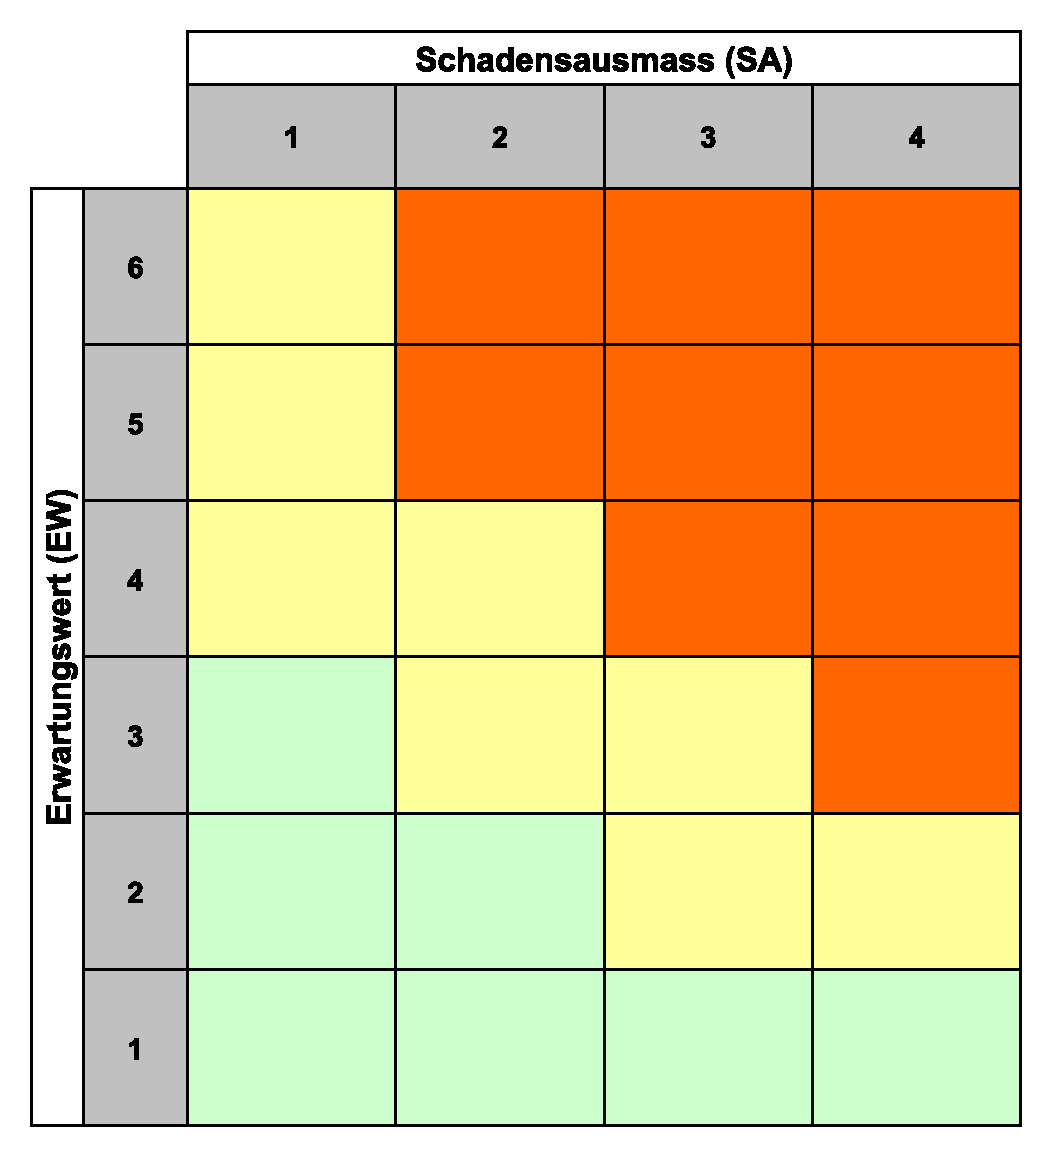
\includegraphics[width=0.75\textwidth]{./Risks_Diagramm/Diagramm_Risiko_allg.pdf}
    \caption{Grafische Darstellung der Risikoanalyse Allgemein}~\label{fig:Diagramm_Risiko_allg}
\end{figure}

% ========= MECHANIK

\subsubsection*{Mechanik}

\begin{table}[H]
    \begin{tabularx}{\textwidth}{|>{\centering\arraybackslash}p{2cm}|>{\raggedright\arraybackslash}X|>{\centering\arraybackslash}p{0.75cm}|}
        \hline
        \textbf{Risiko \#}        & \textbf{Massnahme}
                                  & \textbf{Neu EW}                                                                                                                                                                 \\
        \hline
        \rowcolor{yellow!30}
        2.~\ref{tabrow:risks_2_1} & Höhere Gewichtung auf dieses Detail in der Konzeptbewertung.
                                  & 3                                                                                                                                                                               \\
        \hline
        \rowcolor{green!30}
        2.~\ref{tabrow:risks_2_2} & Gewicht der Bauteile frühzeitig überschlagen und bei jedem Entwicklungsschritt berücksichtigen. Liste für bereits bekannte Gewichte führen und Budget für Baugruppen festlegen.
                                  & 1                                                                                                                                                                               \\
        \hline
    \end{tabularx}
    \caption{Erfasste Massnahmen für die Mechanik betreffende Risiken}~\label{tab:Erfasste_Massnahmen_mech}
\end{table}

Abbildung~\ref{fig:Diagramm_Risiko_mech} zeigt schematisch, wie die getroffenen
Massnahmen entsprechende Risiken für den Projekterfolg reduzieren.

\begin{figure}[h]
    \centering
    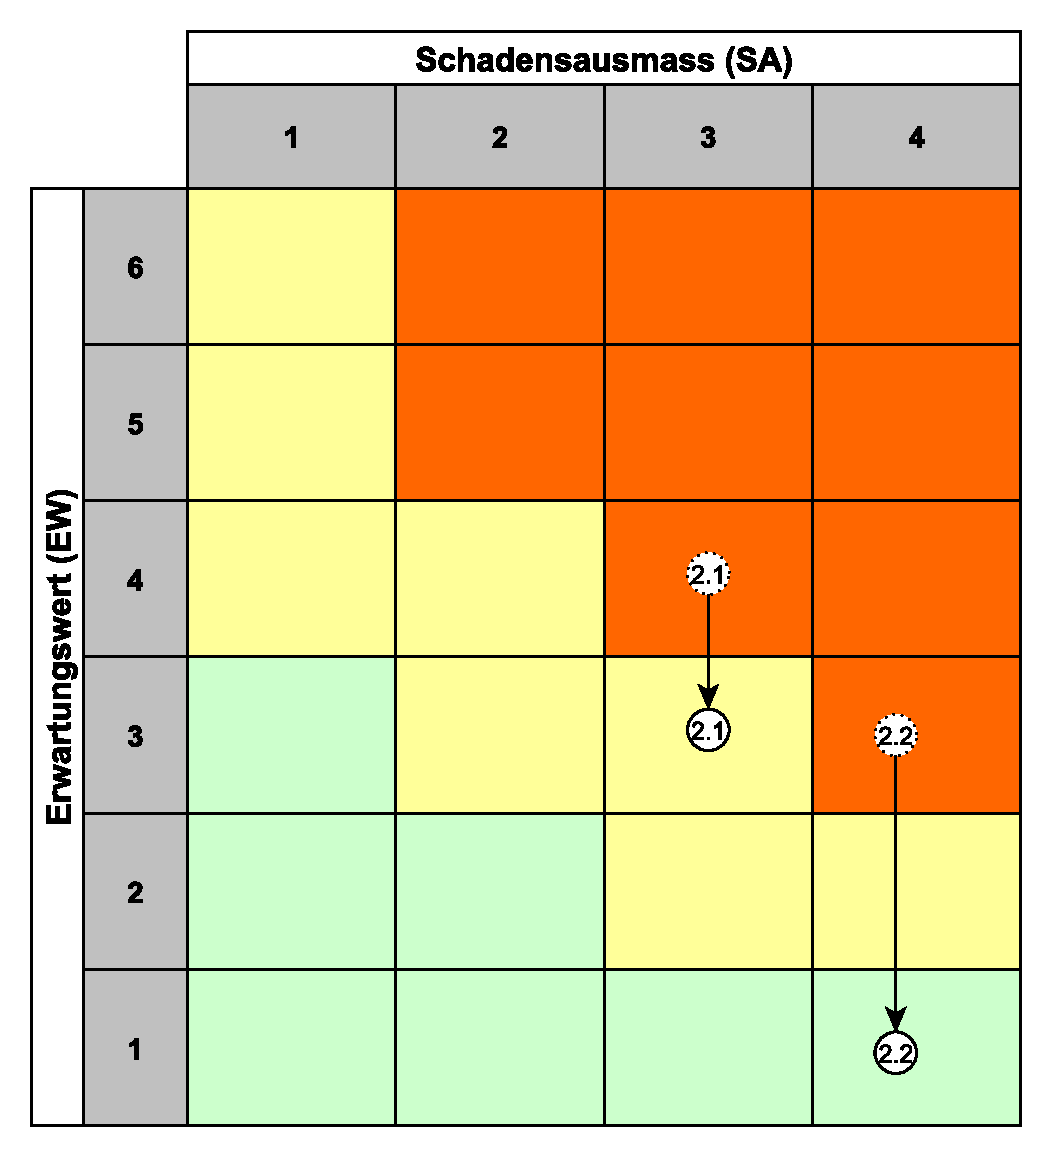
\includegraphics[width=0.75\textwidth]{./Risks_Diagramm/Diagramm_Risiko_mechanik.pdf}
    \caption{Grafische Darstellung der Risikoanalyse Mechanik}
    \label{fig:Diagramm_Risiko_mech}
\end{figure}

% ========= ELEKTRONIK

\subsubsection*{Elektrotechnik}

\begin{table}[H]
    \begin{tabularx}{\textwidth}{|>{\centering\arraybackslash}p{2cm}|>{\raggedright\arraybackslash}X|>{\centering\arraybackslash}p{0.75cm}|}
        \hline
        \textbf{Risiko \#}        & \textbf{Massnahme}
                                  & \textbf{Neu EW}                                                                                                                                                                                             \\

        \hline
        \rowcolor{yellow!30}
        3.~\ref{tabrow:risks_3_1} & Frühzeitiges Testen und Optimieren der Genauigkeit der Sensorik. Möglichkeit bieten, das Fahrzeug nach Fahrzeugwinkel und gefahrenen Strecken zu regeln. Technologieentscheid erst nach ausgiebigem Testen.
                                  & 2                                                                                                                                                                                                           \\

        \hline
        \rowcolor{yellow!30}
        3.~\ref{tabrow:risks_3_2} & Sensorik, die optisch arbeitet, möglichst abgekapselt von der Umwelt betreiben. Alternativ Wellenlängen, die das sichtbare Licht beinhalten, vermeiden.
                                  & 3                                                                                                                                                                                                           \\

        \hline
        \rowcolor{green!30}
        3.~\ref{tabrow:risks_3_3} & Akku doppelt herstellen/einkaufen, Ladestation extern ausführen, um immer einen vollgeladenen Akku bereit zu haben.
                                  & 1                                                                                                                                                                                                           \\

        \hline
        \rowcolor{green!30}
        3.~\ref{tabrow:risks_3_4} & Kommunikationsleitungen mindestens als Twisted-Pairs mit GND – besser aber geschirmt ausführen.
                                  & 1                                                                                                                                                                                                           \\

        \hline
        \rowcolor{yellow!30}
        3.~\ref{tabrow:risks_3_5} & Genügend Spannungsreserve des Akkus „nach oben“ einplanen. Vor der Spannungsversorgung für High-Level-Controller und Mikrocontroller aktive Filter (z.B. LDO oder ähnliches) vorsehen.
                                  & 2                                                                                                                                                                                                           \\
        \hline

    \end{tabularx}
    \caption{Erfasste Massnahmen für Risikoanalyse}~\label{tab:Erfasste_Massnahmen_elektro}
\end{table}

Abbildung~\ref{fig:Diagramm_Risiko_elektro} zeigt schematisch auf, wie die
getroffenen Massnahmen entsprechende Risiken auf den Projekterfolg reduzieren.

\begin{figure}[h]
    \centering
    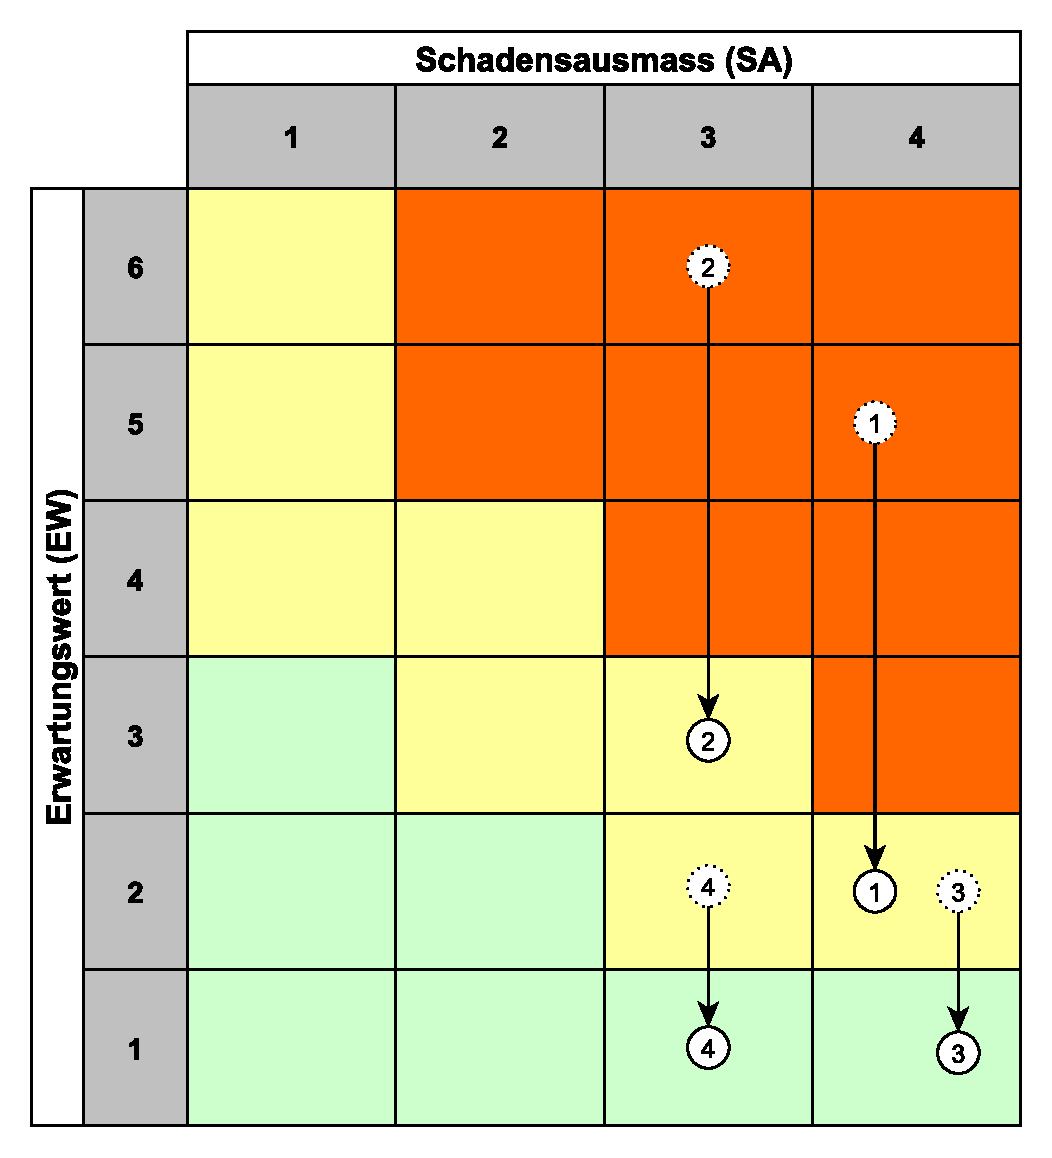
\includegraphics[width=0.75\textwidth]{./Risks_Diagramm/Diagramm_Risiko_elektro.pdf}
    \caption{Grafische Darstellung Risikoanalyse Elektrotechnik}~\label{fig:Diagramm_Risiko_elektro}
\end{figure}

% ========= INFORMATIK

\subsubsection*{Informatik}

\begin{table}[H]
    \begin{tabularx}{\textwidth}{|>{\centering\arraybackslash}p{2cm}|>{\raggedright\arraybackslash}X|>{\centering\arraybackslash}p{0.75cm}|}
        \hline
        \textbf{Risiko \#}        & \textbf{Massnahme}
                                  & \textbf{Neu EW}                              \\

        \hline
        \rowcolor{yellow!30}
        4.~\ref{tabrow:risks_4_1} & Fallback-Lösung: Fahrzeug fährt immer links.
                                  & 3                                            \\

        \hline

    \end{tabularx}
    \caption{Erfasste Massnahmen für Risikoanalyse}~\label{tab:Erfasste_Massnahmen_info}
\end{table}

Abbildung~\ref{fig:Diagramm_Risiko_info} zeigt schematisch auf, wie die
getroffenen Massnahmen entsprechende Risiken auf den Projekterfolg reduzieren.

\begin{figure}[h]
    \centering
    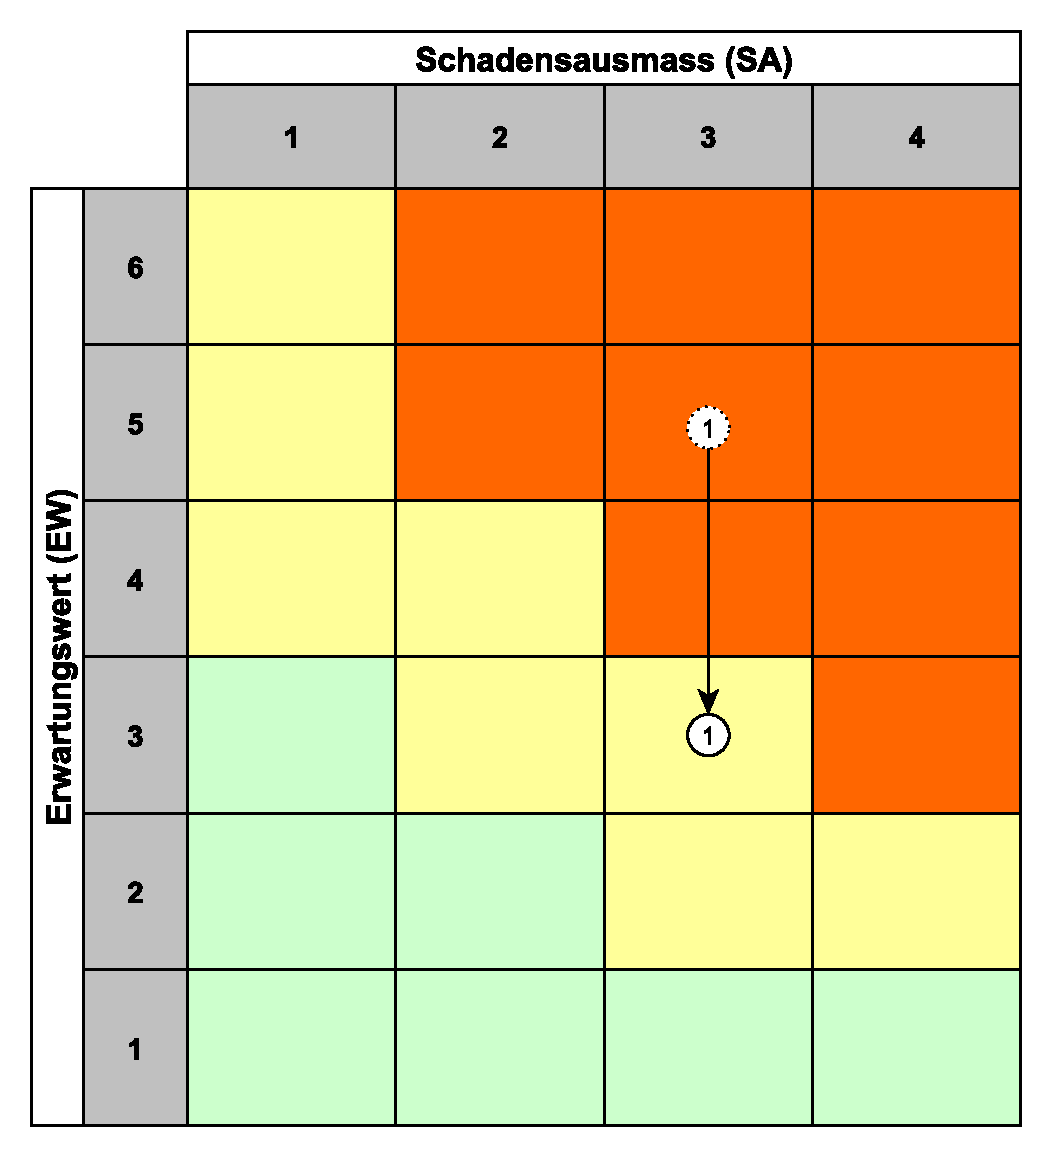
\includegraphics[width=0.75\textwidth]{./Risks_Diagramm/Diagramm_Risiko_info.pdf}
    \caption{Grafische Darstellung Risikoanalyse Informatik}~\label{fig:Diagramm_Risiko_info}
\end{figure}

\end{document}
